% Overleaf: XeLaTeX. English version; both manuscripts use the same results.
\documentclass[10pt,journal,compsoc]{IEEEtran}
\usepackage{fontspec}
\usepackage{fix-cm}
\setmainfont{texgyrepagella-regular.otf}[BoldFont=texgyrepagella-bold.otf,ItalicFont=texgyrepagella-italic.otf,BoldItalicFont=texgyrepagella-bolditalic.otf]
\setsansfont{texgyreheros-regular.otf}[BoldFont=texgyreheros-bold.otf,ItalicFont=texgyreheros-italic.otf,BoldItalicFont=texgyreheros-bolditalic.otf]
\setmonofont{lmmono10-regular.otf}
\usepackage{amsmath,amssymb,amsthm,graphicx,booktabs}
\usepackage{algorithm,algpseudocode,cite}
\usepackage[hidelinks]{hyperref}
\newtheorem{theorem}{Theorem}
\graphicspath{{figures/}}
\newcommand{\NaiveSmall}{0.3963}
\newcommand{\SlideSmall}{0.0310}
\newcommand{\NaiveMedium}{2.8641}
\newcommand{\SlideMedium}{0.0975}
\newcommand{\NaiveLarge}{31.3657}
\newcommand{\SlideLarge}{0.3098}

\begin{document}
\title{Transcript-Guided Sliding-Window Selection\\for Long-Form Speech Retrieval}
\author{Author Name (replace before submission)\thanks{Algorithm course paper. Experiments evaluate key-span retrieval using public SPIRAL transcript annotations.}}
\markboth{Algorithm Design and Analysis: Course Paper}{Transcript-Guided Sliding-Window Selection}
\IEEEtitleabstractindextext{%
\begin{abstract}
Relevant information in a long recording often occurs within a local passage. Inspired by the information-selection problem studied in SpeechPrune, this paper examines a simple transcript-guided approach: compute TF-IDF cosine relevance between a question and each transcript sentence, then select the fixed-length contiguous window with the largest total score. A running-sum update finds the optimal window in $O(N)$ time with $O(1)$ auxiliary workspace once scores are available. We give a loop-invariant proof and evaluate the method on all 1,012 public SPIRAL transcript records against first-window cropping, a uniform random window, and score top-$k$. At a nominal 20\% sentence budget, the sliding window achieves an 86.86\% full key-span hit rate, compared with 25.30\% for a random window and 87.06\% for top-$k$. It always retains one contiguous passage, whereas top-$k$ retains 2.68 passages on average. At a 50\% budget, the respective hit rates are 96.44\% and 94.37\%. These results characterize how the continuity constraint interacts with evidence coverage across budgets. Evaluation uses supplied transcripts and sentence-count budgets.
\end{abstract}
\begin{IEEEkeywords}
Long-form speech retrieval, sliding window, contiguous segment selection, TF-IDF, SPIRAL, algorithm analysis.
\end{IEEEkeywords}}
\maketitle
\IEEEdisplaynontitleabstractindextext
\IEEEpeerreviewmaketitle

\section{Introduction}
Retrieving a specific detail from a meeting, lecture, or conversation is a common requirement in long-form speech understanding. A question about the time of a meeting, for example, may depend on a single sentence within a much longer recording. SpeechPrune formulates a speech information retrieval task, introduces the SPIRAL benchmark, and selects audio tokens to reduce the amount of information passed to subsequent processing\cite{lin2025speechprune}.

Segment selection must account for both relevance and continuity. Selecting individually high-scoring positions can produce a fragmented sequence. A contiguous crop preserves the original order within one interval. We study this choice with an implementation whose individual operations are easy to inspect: assign a score to every transcript sentence and scan the sequence with a fixed-length window.

Our research question is: \emph{Under the same sentence-count budget, how often does the maximum-score contiguous window retain the annotated key span, and how does it compare with noncontiguous score top-$k$ selection?} To isolate the selection algorithm, we use the supplied SPIRAL transcript sentences and lexical relevance scores. Questions determine the scores. Answer choices, correct answers, and annotated key positions do not enter scoring.

We provide a linear-time maximum-sum algorithm and proof, compare four selectors on 1,012 records, and verify the implementation through annotation audits and exhaustive scans. TF-IDF and sliding windows are established techniques; this study analyzes the computation and evidence coverage of contiguous selection.

\section{Related Work}
\subsection{Speech Understanding and Relevant Information}
Audio-language models such as Qwen2-Audio combine audio with textual instructions for analysis\cite{chu2024qwen}. SpeechPrune first selects information using audio--question similarity and then applies approximate-attention-based token selection\cite{lin2025speechprune}. Its method already incorporates frame organization and temporal structure. Our study simplifies selection to a contiguous interval of transcript sentences so that every computation can be inspected independently.

Temporal locality is also studied in audio representation compression. Luo et al. merge nearby audio tokens within local temporal windows and report task-dependent locality effects\cite{luo2026locality}. This provides context for examining contiguous and dispersed selection. Our evaluation focuses on annotated evidence coverage at sentence level.

\subsection{Transcript Retrieval and Window Search}
Automatic speech recognition can supply text for a retrieval pipeline; Whisper is a representative speech-recognition system\cite{radford2023whisper}. Once transcripts are available, term weighting and vector similarity provide basic relevance scores\cite{manning2008ir}. Here, supplied reference transcripts keep recognition errors separate from selection errors.

Score-sum optimality and key-span coverage are distinct evaluation levels, examined through proof and dataset experiments, respectively.

\section{Problem Definition and Relevance Scoring}
\subsection{Inputs, Budget, and Objective}
Let $X=(x_1,\ldots,x_N)$ be transcript sentences in recording order, $q$ the question, and $s_1,\ldots,s_N$ their relevance scores. A budget $k$, with $1\le k\le N$, specifies the number of retained sentences. The window starting at $t$ is
\begin{equation}
 W_t=\{t,t+1,\ldots,t+k-1\},\quad 1\le t\le N-k+1.
\end{equation}
The selected start maximizes the total score:
\begin{equation}
 t^*=\arg\max_t F(t),\qquad F(t)=\sum_{i=t}^{t+k-1}s_i.
 \label{eq:target}
\end{equation}
The mathematical definition resolves ties in favor of the earliest start. Since every candidate contains $k$ sentences, maximizing the sum also maximizes the mean score.

The controlled budget is sentence count. Sentence lengths and speaking durations vary, so an equal $k$ does not imply equal seconds or equal audio-token counts. We additionally record the retained lexical word fraction to describe this distinction.

\subsection{Training-Free Sentence Scores}
We use TF-IDF weighting and cosine similarity\cite{manning2008ir}. Each recording has its own vocabulary and document frequencies, treating its sentences as documents. If term $v$ occurs in $\mathrm{df}(v)$ sentences, its smoothed inverse document frequency is
\begin{equation}
 \mathrm{idf}(v)=1+\log\frac{N+1}{\mathrm{df}(v)+1}.
\end{equation}
For a positive count $c(v,x)$ in text $x$, the unnormalized weight is
\begin{equation}
 z_v(x)=[1+\log c(v,x)]\,\mathrm{idf}(v).
\end{equation}
Sentence and question vectors are normalized independently, giving
\begin{equation}
 s_i=\frac{z(x_i)^\top z(q)}{\|z(x_i)\|_2\|z(q)\|_2}.
 \label{eq:score}
\end{equation}
A zero vector receives a zero similarity. Preprocessing lowercases text, extracts alphabetic words and numbers, and removes the fixed stopword list distributed with the code. We use neither stemming nor a semantic model. Question terms absent from the current transcript vocabulary are omitted. All four selectors receive identical scores.

\section{Sliding-Window Algorithm and Analysis}
\subsection{Update Rule and Worked Example}
Enumerating each window and recomputing its sum costs $O((N-k+1)k)$ time. Consecutive windows share $k-1$ entries, permitting the update
\begin{equation}
 F(t+1)=F(t)-s_t+s_{t+k}.
 \label{eq:update}
\end{equation}
After summing the first window, the algorithm subtracts the score leaving the interval and adds the entering score.

For scores $(1,2,8,9,7,1)$ and $k=3$, the window sums are 11, 19, 24, and 17. The selected interval contains positions 3--5 and has total score 24. This numerical example illustrates the update and is separate from the dataset evaluation.

\begin{algorithm}[t]
\caption{Maximum-score fixed-sentence window}\label{alg:window}
\begin{algorithmic}[1]
\Require Scores $s_1,\ldots,s_N$; budget $k$
\Ensure Best start $t^*$ and window sum $b$
\State Check $1\le k\le N$
\State $c\gets\sum_{i=1}^{k}s_i$; $b\gets c$; $t^*\gets1$
\For{$t=2,\ldots,N-k+1$}
 \State $c\gets c-s_{t-1}+s_{t+k-1}$
 \If{$c>b$}
  \State $b\gets c$; $t^*\gets t$
 \EndIf
\EndFor
\State \Return $(t^*,b)$
\end{algorithmic}
\end{algorithm}

\subsection{Correctness}
\begin{theorem}
Under exact arithmetic, Algorithm~\ref{alg:window} returns an optimal window for~\eqref{eq:target}, choosing the earliest start when several windows are optimal.
\end{theorem}
\begin{proof}
We maintain two invariants after processing window $t$: $c=F(t)$, and $b$ is the largest sum among all processed windows, with $t^*$ its earliest maximizing start.

Initialization explicitly computes the first window sum, establishing both invariants. Equation~\eqref{eq:update} updates $c$ to the next window sum. A strictly larger value replaces $b$ and its start; otherwise the previous record is retained. The strict comparison preserves the earlier start on ties, so both invariants continue to hold.

On termination, all $N-k+1$ legal windows have been processed. Thus $b$ is the global maximum, and $t^*$ satisfies the stated tie rule.
\end{proof}

\subsection{Complexity and Implementation Scope}
Initialization takes $O(k)$ time, followed by $N-k$ constant-time updates, for a total of $O(N)$. Current sum, best sum, and best start require $O(1)$ auxiliary workspace, excluding the input scores and returned sentences. The implementation initializes the sum by indexed iteration rather than by copying a length-$k$ slice.

Text reading and TF-IDF feature construction occur before window selection; their costs depend on token counts and vocabulary size. The linear-time result concerns selection after scoring. Timing experiments use the same boundary and compare naive recomputation with incremental updates.

For $k=1$, the algorithm selects a highest-scoring sentence. For $k=N$, it selects the complete transcript. Initialization from the first legal window also handles all-negative score sequences. The experimental scores are nonnegative, but the proof does not require this property.

\section{Experimental Design}
\subsection{Dataset and Annotation Audit}
We evaluate all 1,012 public SPIRAL records\cite{lin2025speechprune}: 350 lectures, 324 meetings, and 338 conversations. SPIRAL uses generated dialogue and synthesized speech. We use its reference transcripts, questions, and key-span annotations.

The released combined-audio sentence lists define sequence order. Key-sentence indices are interpreted as zero-based half-open intervals. All 1,012 intervals satisfy the index bounds. Records contain 6--34 sentences, with a mean of 17.06. Key spans contain one sentence in 891 records and two sentences in 121 records.

After normalization, span text exactly matches the original key sentence in 924 records, contains it with extra material in 79, and falls into neither category in nine. The main experiment preserves all records and the published span indices. A sensitivity analysis reports results on the 924 exact-match records without manually relocating labels.

\subsection{Budgets and Selectors}
For each record, nominal ratios are $\rho\in\{0.1,0.2,0.3,0.5\}$, with $k=\lceil\rho N\rceil$. All four selectors retain the same sentence count. First-window cropping retains the first $k$ sentences. Random-window cropping samples a legal contiguous start uniformly. Score top-$k$ retains the $k$ highest-scoring sentences in original order. The sliding window optimizes~\eqref{eq:target}.

For the random baseline, we enumerate every legal start and calculate exact expected metrics, eliminating Monte Carlo variation. Top-$k$ resolves equal scores by sentence order. Budget ratios are fixed in advance; answers and key positions do not tune the selectors.

\subsection{Metrics and Verification}
Let $G$ denote annotated key-sentence indices and $S$ selected indices. The primary metric is full key-span hit rate:
\begin{equation}
 H=\frac{1}{M}\sum_{j=1}^{M}\mathbf{1}[G_j\subseteq S_j],
\end{equation}
where $M=1012$. The random baseline averages per-record expected hit probabilities. Additional outputs include any-span hit rate, gold-sentence recall, selected score sum, and the number of contiguous runs, defined using adjacency of selected indices.

Sentence retention is $k/N$. Lexical word retention counts preprocessed words in selected sentences relative to the complete transcript, using the scoring tokenizer. These quantities describe retained input size; hit rate measures evidence retention rather than final answer accuracy.

The implementation uses Python 3.13.15 and NumPy 2.5.3. Verification compares 2,000 random integer arrays with independent exhaustive window scans and checks the objective value for all $1012\times4=4048$ record--budget combinations, using a floating-point tolerance of $10^{-10}$. Timing uses random score arrays of length 1,000, 3,000, and 10,000 with $k=N/10$. Each method is warmed up once; we report the median of seven calls.

\section{Results and Analysis}
\subsection{Key-Span Retention}
Table~\ref{tab:main} reports full key-span hit rates for all budgets. Sliding-window selection exceeds first-window and random-window cropping at every tested ratio. At the nominal 20\% budget, its hit rate is 86.86\%, compared with 25.30\% for the random baseline, a difference of 61.56 percentage points. Question-dependent relevance scores thus concentrate retained evidence on this dataset.

\begin{table}[t]
\caption{Full key-span hit rate (\%) on all 1,012 records. Budgets are nominal sentence ratios; every method uses the same per-record $k$. Random-window values are exact expectations.}
\label{tab:main}
\centering\footnotesize
\setlength{\tabcolsep}{4pt}
\begin{tabular}{lrrrr}
\toprule
Method & 10\% & 20\% & 30\% & 50\%\\

\midrule
First & 1.88 & 11.07 & 29.74 & 70.75\\
Random window & 12.59 & 25.30 & 39.86 & 67.62\\
Score top-$k$ & 80.34 & 87.06 & 89.72 & 94.37\\
Sliding window & 80.04 & 86.86 & 91.01 & 96.44\\
\bottomrule
\end{tabular}

\end{table}

Compared with score top-$k$, the sliding window is lower by 0.30 and 0.20 percentage points at 10\% and 20\%, and higher by 1.28 and 2.08 points at 30\% and 50\%. These are descriptive dataset differences. Larger windows have more capacity to cover adjacent key sentences; top-$k$ optimizes individual sentence scores.

\begin{figure*}[t]
\centering
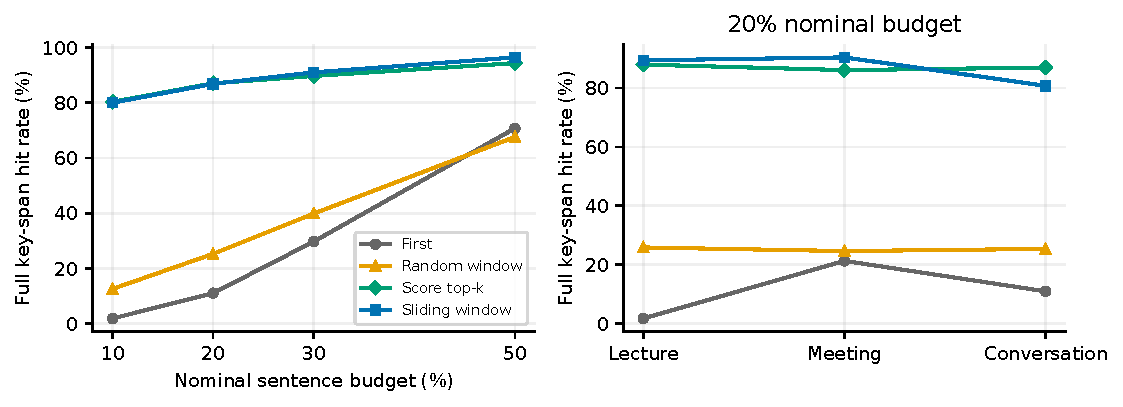
\includegraphics[width=0.94\textwidth]{retrieval.pdf}
\caption{Left: full key-span hit rate across nominal sentence budgets. Right: results by scenario at a 20\% budget. All selectors share TF-IDF scores; the random baseline averages all legal contiguous starts exactly.}
\label{fig:retrieval}
\end{figure*}

\subsection{Continuity and Scenario Differences}
At the 20\% budget, sliding-window hit rates for lectures, meetings, and conversations are 89.43\%, 90.43\%, and 80.77\%. The corresponding top-$k$ rates are 88.00\%, 86.11\%, and 86.98\%. The effect of continuity varies across scenarios, with lower coverage than dispersed selection on conversations.

The sliding window always returns one contiguous passage. Top-$k$ returns 2.68 passages on average at this budget. Mean selected score sums are 0.7177 and 0.8924, respectively. Top-$k$ has the higher sum, as expected from its unconstrained selection objective; a higher score sum does not guarantee a higher full-span hit rate at every budget. Figure~\ref{fig:example} shows the first record in dataset order, specified independently of method performance.

\begin{figure}[t]
\centering
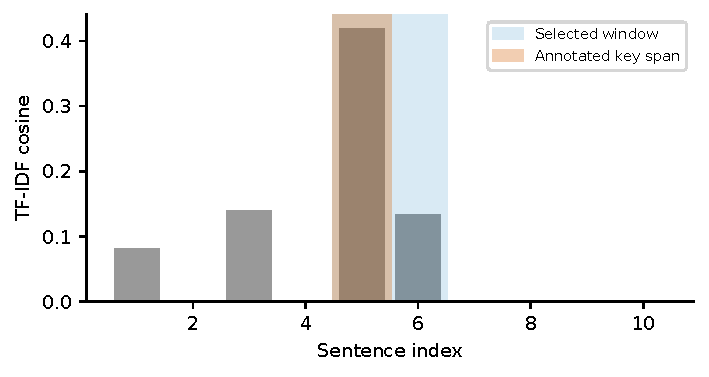
\includegraphics[width=\columnwidth]{example.pdf}
\caption{Sentence scores, selected window, and annotated key span for \texttt{lecture\_0} at the nominal 20\% budget. Blue marks the selected interval; orange marks the annotated span.}
\label{fig:example}
\end{figure}

\subsection{Budget Interpretation and Annotation Sensitivity}
Rounding makes the actual mean sentence retention 22.47\% at the nominal 20\% budget. At that setting, sliding windows retain 25.25\% of lexical words on average, compared with 28.25\% for top-$k$. Equal sentence counts therefore leave differences in input length because sentence lengths vary.

On the 924 exact-text-match records, hit rates at 20\% are 86.90\% for the sliding window, 87.23\% for top-$k$, and 25.31\% for a random window. The principal ordering resembles that of the full dataset. A record-level annotation audit accompanies the implementation.

\subsection{Correctness and Selection Cost}
All 2,000 integer-array comparisons agree exactly with exhaustive scanning in both optimal sum and start index. All 4,048 real record--budget combinations pass the objective-value check. For lengths 1,000, 3,000, and 10,000, median sliding-update times are \SlideSmall, \SlideMedium, and \SlideLarge\ ms; naive scanning takes \NaiveSmall, \NaiveMedium, and \NaiveLarge\ ms. Measurements use one Windows 11 machine with an Intel Family 6 Model 183 CPU and include only selection after score generation.

The timings follow the complexity analysis. When $k=N/10$ grows with input size, repeated naive summation performs approximately quadratic work, while incremental updates keep a linear scan. This comparison explains the implementation cost of window search. Transcription and language-model inference require separate measurements in a complete system.

\section{Discussion and Application Scope}
The method targets localized evidence; distant evidence may require multiple windows. Lexical matching has limited support for paraphrases and cross-sentence reasoning. Sentence embeddings or audio--text alignment could replace the scores, with retrieval effectiveness evaluated again.

The empirical study uses reference transcripts and executes neither ASR nor an audio-language model. Mapping selections back to recordings requires sentence timestamps. Fixed-second budgets require equal-duration blocks or timestamp intervals. End-to-end answer accuracy, audio-splicing effects, and inference speed require corresponding system experiments.

\section{Conclusion}
Motivated by the retrieval setting in SpeechPrune, this paper studies transcript-guided contiguous segment selection as a fixed-length maximum-sum search. A loop invariant proves optimality for given scores, with linear-time selection. On 1,012 SPIRAL records, the method achieves an 86.86\% full key-span hit rate at a nominal 20\% sentence budget while retaining one contiguous passage. Comparisons with top-$k$ vary across budgets and scenarios, showing why continuity and evidence coverage should be evaluated jointly. The resulting course study combines simple scoring, array updates, and reproducible evaluation.

\section*{Reproducibility and Assistance}
The project includes a public-annotation downloader, the window algorithm, four selectors, record-level results, annotation audits, and plotting code. All numerical results were computed by the supplied program. Generative AI assisted research organization, code, and manuscript preparation; the submitting author should verify the work and report assistance according to course requirements.
\bibliographystyle{IEEEtran}
\bibliography{references}
\end{document}
